
\chapter{System Architecture}



\noindent Figure 3.1 illustrates the system architecture for the ASTRO Platform, designed to support small-scale vendors by facilitating bulk order discounts, demand forecasting, and logistics optimisation. This architecture provides a clear overview of the platform’s components and how they work together to streamline the entire process from order initiation to optimized delivery. Here’s a breakdown of the key aspects and importance of this architecture:

\begin{figure}[h]
    \centering
    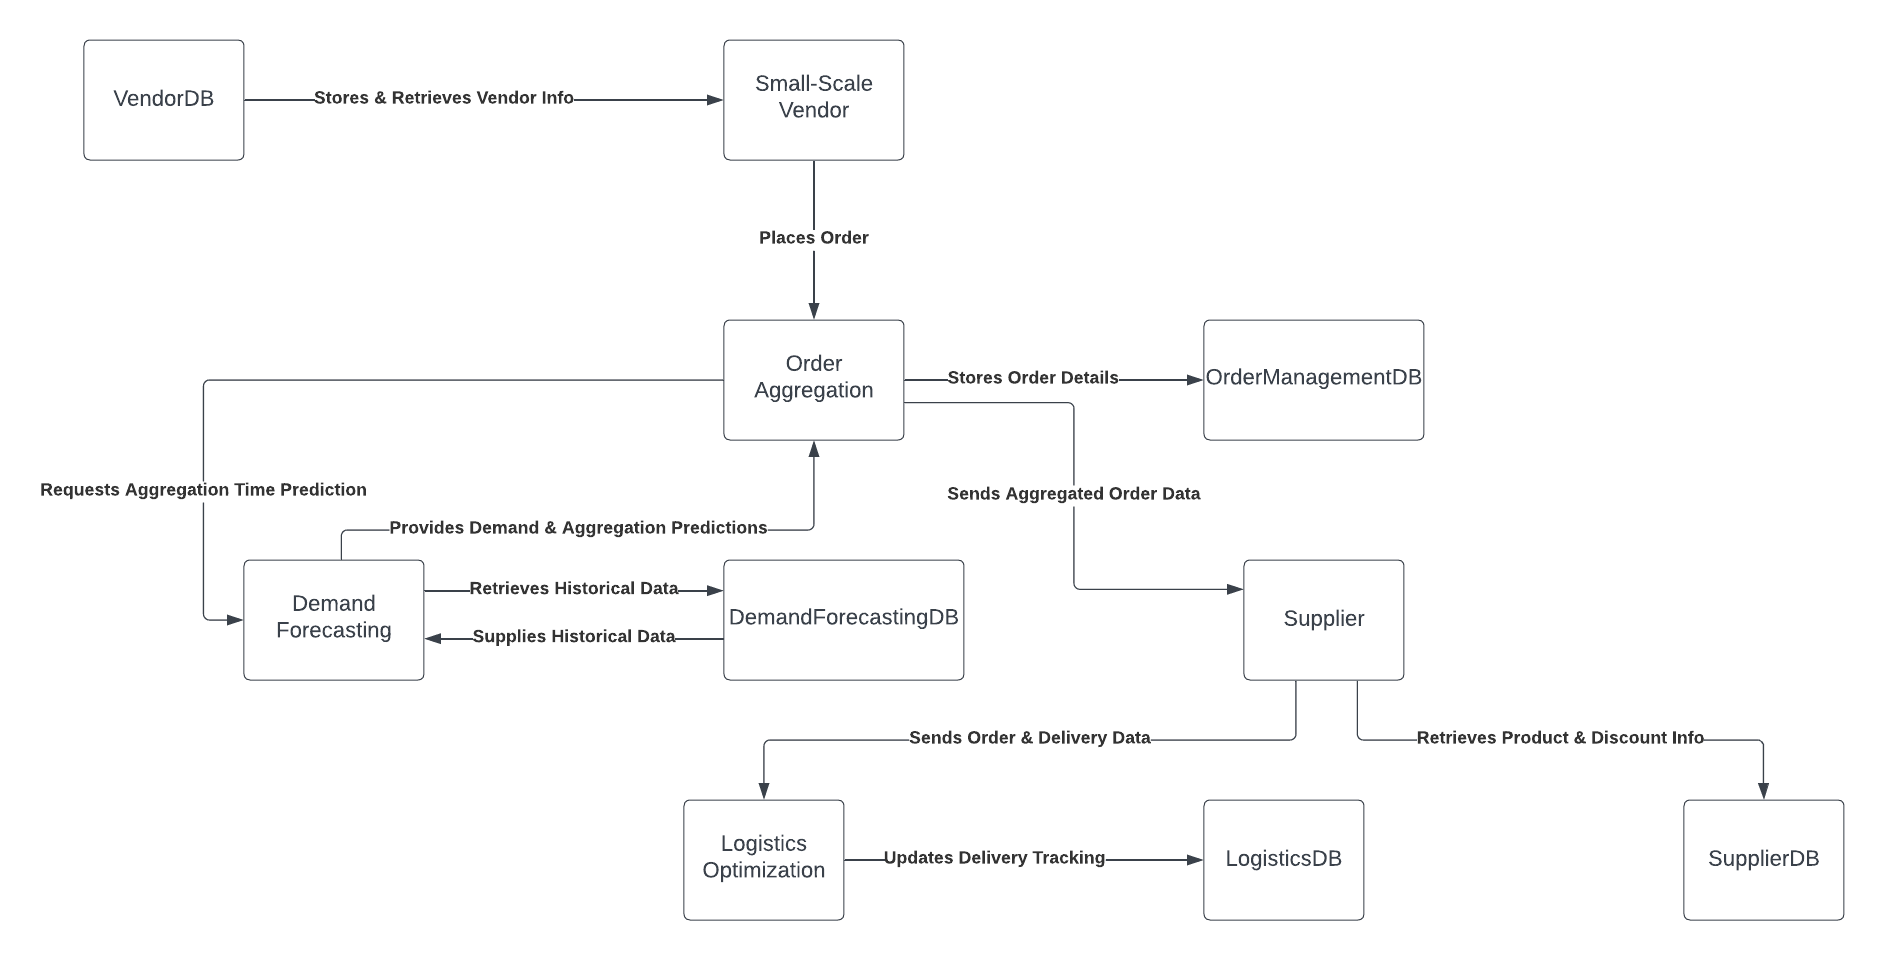
\includegraphics[width=\textwidth]{Figures/system_archh.png}
    \caption{System Architecture}
    \label{fig:architecture}
\end{figure}


\begin{enumerate}
    \item \textbf{High-Level Overview:} The architecture serves as a roadmap, showing the main stages of the platform’s workflow. From initial product viewing and order placement by vendors, through demand forecasting, order aggregation, and logistics optimisation, this high-level overview provides all stakeholders—including vendors, suppliers, and platform administrators—with a clear understanding of the system’s core functionality.

    \item \textbf{Clarifies Data Flow:} The architecture clarifies the flow of data within the system, beginning with the acquisition of order and sales data. This data undergoes preprocessing and feature extraction, followed by demand forecasting with the Neural Prophet model. The forecast data then flows into the Order Aggregation module, which combines vendor orders to meet bulk purchase thresholds. Finally, optimized delivery routes are created through the Logistics Optimisation module, using Green Routing techniques. This sequential data flow enhances system transparency and makes it easy to identify potential bottlenecks.

    \item \textbf{Enables Collaborative Order Aggregation:} The architecture highlights how order aggregation enables small-scale vendors to achieve bulk discounts. By aggregating orders from multiple vendors, the platform ensures Minimum Order Quantities (MOQs) are met, enabling vendors to access bulk discounts typically reserved for larger chains. This aspect of the system is crucial for enhancing the competitiveness of small vendors.

    \item \textbf{Supports Logistics Optimisation through Green Routing:} The architecture emphasizes the logistics optimisation approach used in the platform. The Green Routing component incorporates route flexibility and service time windows to create efficient and environmentally friendly delivery routes. This optimisation minimizes transportation costs and enhances delivery reliability for vendors, contributing to a streamlined and cost-effective supply chain.

    \item \textbf{Enables Real-Time Notifications and Updates:} The system architecture includes a notification mechanism that provides real-time updates to vendors on order status, inventory levels, and logistics. These notifications foster transparency, enabling vendors to make informed decisions about inventory and delivery schedules.

    \item \textbf{Facilitates Collaboration and Communication Among Stakeholders:} The system architecture acts as a shared framework, providing a common language for platform users, developers, and suppliers. It allows stakeholders to better understand the interactions between components and collaborate effectively toward improving platform functionality. This collaborative framework is essential for ensuring smooth operations and adapting to vendor needs.

\end{enumerate}

\noindent Overall, the system architecture is crucial for understanding the ASTRO Platform. It provides a clear visual representation of the platform’s workflow, highlighting key features such as order aggregation, demand forecasting, logistics optimisation, and real-time notifications. These components work together to enhance vendor competitiveness by offering cost-saving opportunities, efficient delivery solutions, and improved collaboration with suppliers.

\section{Dataset}


\textbf{Purpose:} This dataset supports research in sales forecasting, specifically at the item and store levels. The objective is to predict the next three months of sales for individual items at various store locations, applicable for demand forecasting, inventory management, and sales optimisation.

\textbf{Data Collection:} This dataset was collected from multiple store locations, representing real-world sales data with variations in store performance and item demand. It provides diverse daily sales records for individual items across different stores, enabling demand pattern analysis.

\textbf{Data Fields:}
\begin{description}
    \item[\textbf{date:}] Date of each sale record. There are no adjustments for holidays or store closures, simplifying the analysis but possibly requiring external data for event-based effects.
    \item[\textbf{store:}] A unique identifier for each store, allowing for store-level analysis and capturing unique characteristics and item demand differences.
    \item[\textbf{item:}] A unique identifier for each item sold, enabling item-level demand forecasting and cross-store analysis.
    \item[\textbf{sales:}] The number of items sold at a particular store on a given date, which is the target variable for forecasting models.
\end{description}

\textbf{File Descriptions:}
\begin{description}
    \item[\textbf{train.csv:}] Contains historical sales data used for training forecasting models.
    \item[\textbf{test.csv:}] Provides the test data where future sales predictions are needed, with a time-based split for realistic scenario testing.
    \item[\textbf{sample\_submission.csv:}] A sample submission file showing the required format for submitting sales forecasts.
\end{description}

\textbf{Usage in Research:} This dataset supports the development and validation of time series forecasting models. It allows researchers to explore seasonality, trends, and external influences on sales. Models like Neural Prophet or ARIMA can be applied, along with machine learning techniques for enhanced forecasting accuracy.

\textbf{Challenges and Opportunities:} Although the dataset lacks explicit holiday or store event information, researchers may incorporate external data to improve forecasts. This provides an opportunity to explore techniques that account for seasonality and trend modelling, such as Fourier series for seasonality or external regressors.

\textbf{Access:} This dataset is easily accessible, enabling collaborative studies on sales forecasting and providing a resource for testing and improving demand forecasting algorithms.


\section{Preprocessing Steps}

To ensure the data is prepared for accurate demand forecasting and that the model interprets the features effectively, the following preprocessing steps are applied:

\subsection*{Tasks}

\textbf{Handling Missing Values:} Missing data may exist in historical datasets due to reporting errors or system downtime. The Neural Prophet model employs a data imputation mechanism to avoid excessive data loss when working with incomplete data. Missing events are filled in with zeros, indicating their absence. For other real-valued variables, including the time series itself (when autoregression is enabled), the following imputation procedure is applied:

\begin{enumerate}
    \item \textbf{First Step:} Missing values are approximated using bi-directional linear interpolation. The missing values are filled by interpolating between the last known value before and after the missing data. This process is applied to a maximum of 5 missing values in each direction.
    \item \textbf{Second Step:} Remaining missing values are imputed using a centered rolling average. A window of 30 is used, and up to 20 consecutive missing values can be filled.
    \item \textbf{Third Step:} If more than 30 consecutive missing values remain, these data points are dropped from the dataset.
\end{enumerate}

This imputation process ensures minimal loss of data while maintaining the integrity of the time series.

\textbf{Scaling and Normalization:} To improve model efficiency, numerical features, particularly sales data, are normalized. The Neural Prophet model offers various normalization options, with the default being the soft method. This approach scales the minimum value to 0.0 and the 95th quantile to 1.0, ensuring that the time series values are appropriately transformed for the model.

The formula for soft normalization is as follows:

\[
    x' = \frac{x - \min(x)}{Q_{95} - \min(x)}
\]

where \( Q_{95} \) represents the 95th quantile of the time series values.

\textbf{Time-Based Feature Engineering:} To capture temporal and seasonal patterns in the data, key features like Day of the Week, Month, and a binary IsWeekend indicator are created. These features help the model understand weekly sales patterns, broader seasonal trends (e.g., holiday spikes), and the impact of weekends on sales. The IsWeekend feature is binary, set to 1 if the date is a Saturday or Sunday and 0 otherwise.

\textbf{Lagged Sales Features:} Since past sales are directly predictive of future demand, lagged sales features are created for the last 7 and 30 days to capture both short-term and longer-term patterns. Additionally, rolling statistics such as the rolling mean and rolling standard deviation over the past 30 days are computed. These features smooth out fluctuations and help the model capture trends more accurately. The rolling mean is calculated as:

\[
    \text{Rolling Mean}_{30} = \frac{1}{30} \sum_{i=t-30}^{t-1} \text{Sales}(i)
\]

and the rolling standard deviation as:

\[
    \text{Rolling Std}_{30} = \sqrt{\frac{1}{30} \sum_{i=t-30}^{t-1} (\text{Sales}(i) - \text{Rolling Mean}_{30})^2}
\]


\subsection*{Output}

The result of these preprocessing steps is a clean, normalized dataset with imputed missing values and encoded categorical features. The dataset is now ready for model training, ensuring that the features are aligned and consistent, helping the model make accurate demand forecasts.

\section{Feature Extraction}

Feature extraction is a critical process in the ASTRO platform as it transforms raw sales data into meaningful representations, enabling accurate demand forecasting and efficient operational management. By identifying and engineering relevant features from the dataset, we capture essential patterns, trends, and relationships that enhance the performance of predictive models.

In the context of the dataset, which contains store-level and item-level sales information over time, feature extraction is designed to uncover temporal patterns, historical dependencies, and interactions between stores and items. The extracted features are categorized into two major types: time-based features and lagged variables, both of which are integral to understanding and predicting demand fluctuations.

\subsection{Time-Based Features}

Time-based features play a crucial role in capturing cyclical and seasonal patterns inherent in sales data. By decomposing the date field into granular components, these features allow the model to understand how sales vary across different times of the week, month, and year. For instance, the day of the week feature represents weekdays as integers, enabling the model to differentiate between regular weekday and weekend shopping behaviours. Similarly, the month feature identifies seasonal effects that often influence demand, such as increased sales during holiday months or specific seasonal trends for particular items.

Another important time-based feature is the week of the year, which highlights demand patterns recurring annually, such as back-to-school shopping or end-of-year festive sales. Additionally, a binary is weekend feature isolates the typically higher weekend sales from weekday trends, ensuring that the model appropriately weighs these differences when forecasting.

These features collectively form the temporal backbone of the forecasting model, allowing it to detect repeating cycles and shifts in demand driven by the calendar.

\subsection{Lagged Variables}

Lagged variables focus on incorporating historical sales data to enhance the model’s ability to forecast future demand. These features represent the past performance of sales, which is often predictive of future trends. For example, a 1-day lag feature captures the sales volume from the previous day, providing immediate short-term context for the current demand. Similarly, a 7-day lag feature reflects weekly demand patterns by showing the sales from the same day of the prior week, which is especially useful for capturing weekly seasonality.

To understand longer-term patterns, a 30-day lag feature is introduced, representing sales from one month earlier. This helps in identifying recurring monthly trends or evaluating the effectiveness of past promotions. In addition to specific lags, rolling statistical features such as the rolling average (7-day) and rolling standard deviation (7-day) are calculated. These features smooth short-term fluctuations and provide insights into the stability or variability of demand over a week.

A cumulative sales feature further extends this approach by summing all sales up to the current date for a given store-item combination. This feature captures overall sales momentum and growth trends, offering a long-term perspective on performance.

Lagged variables are particularly effective in making the model aware of historical dependencies, enabling it to account for demand inertia, recent trends, and periodic changes.


The combination of time-based features and lagged variables provides a comprehensive representation of the dataset, balancing temporal patterns with historical sales behaviour. These features enable the demand forecasting models to detect and learn from intricate relationships within the data, ensuring robust predictions and informed decision-making for vendors. Through this customized feature extraction approach, the platform empowers small-scale vendors with insights that drive collaborative efficiency and competitiveness.

\section{Project Modules and Their Integration}

ASTRO platform comprises three core modules: Demand Forecasting, Order Aggregation, and Route Optimisation. These modules work in harmony to streamline vendor operations, optimize costs, and enhance efficiency in the supply chain. By integrating these modules, the platform empowers vendors to achieve bulk order discounts, coordinate deliveries, and reduce logistics expenses, creating a collaborative ecosystem that benefits all participants.


\subsection{Order Aggregation Module}

The Order Aggregation Module builds on the insights provided by the demand forecasting module. Once multiple vendors agree to participate in a joint order, this module combines their requirements into a single bulk order. The process ensures that the MOQ thresholds are met, unlocking discounts from suppliers that would be unattainable for individual vendors.

The aggregation process also categorizes and organizes the joint order to ensure that products are distributed efficiently. Each vendor's share of the bulk order is clearly delineated, and the aggregated data serves as input for the subsequent logistics operations.

Notifications play a key role in this module: vendors are informed about the opportunity to join an order and, once confirmed, receive updates about the order status and expected delivery timelines. The module ensures transparency and coordination among vendors, simplifying the process of collective purchasing.

\subsection{Route Optimisation Module}

The Route Optimisation Module is responsible for ensuring efficient delivery of the aggregated orders. After the order is finalized and fulfilled by the supplier, this module uses Green Route Optimisation algorithms to design an optimal delivery route.

Since the joint order often involves multiple vendors located in different areas, the Route optimisation module focuses on clustering delivery locations and minimizing logistics costs. The Route Flexibility and Service Time Window feature ensures that deliveries are scheduled efficiently while adhering to time constraints.

The module optimizes the route for a single vehicle tasked with delivering products to multiple vendors. Factors such as load capacity, distance between vendors, and delivery time windows are considered to achieve the most cost-effective and eco-friendly route. By reducing unnecessary travel and fuel consumption, this module contributes to both financial savings and environmental sustainability.

\subsection{Demand Forecasting Module}

The Demand Forecasting Module lies at the heart of the platform, enabling vendors to predict future sales and order cycles. By analysing historical sales data, the module leverages the Neural Prophet model to identify trends, seasonal patterns, and demand fluctuations. The predictions provide vendors with actionable insights into when and how much to order, ensuring they maintain optimal inventory levels while avoiding overstocking or stockouts.

Additionally, this module facilitates order cycle prediction, which is critical for synchronizing vendor orders. When a vendor places an order with a supplier, the platform uses the demand forecasting output to identify similar demand cycles for other vendors. This allows the platform to notify these vendors about the opportunity to join the order, achieving the Minimum Order Quantity (MOQ) threshold required for bulk discounts. By doing so, the demand forecasting module not only supports individual vendors but also sets the foundation for collective collaboration.


\subsection{Integration of Modules}

The three modules—demand forecasting, order aggregation, and route optimization—work together in a seamless, integrated manner to ensure efficient operations:

\begin{itemize}
    \item \textbf{Demand Forecasting to Order Aggregation}: The demand forecasting module predicts when vendors are likely to need specific products. When a vendor places an order, the platform cross-references the forecast data to identify other vendors with overlapping demand cycles. Notifications are sent to these vendors, encouraging them to join the order and achieve bulk discounts.
    \item \textbf{Order Aggregation to Route Optimisation}: Once vendors confirm their participation, the order aggregation module compiles their requests into a single bulk order. The aggregated data, including vendor locations and product quantities, is passed to the Route optimisation module.
    \item \textbf{Route Optimisation for Delivery}: The Route optimisation module designs a delivery route to ensure that all vendors receive their products efficiently. The vehicle carrying the bulk order is routed through clustered vendor locations, minimizing travel distance and logistics costs.
\end{itemize}



The seamless integration of demand forecasting, order aggregation, and route optimisation modules creates a powerful, collaborative platform that addresses the challenges faced by small-scale vendors. The demand forecasting module drives proactive order management, the order aggregation module facilitates cost-effective purchasing, and the route optimisation module ensures efficient delivery. Together, these modules enable vendors to compete with large retail chains by reducing costs, improving operations, and fostering a cooperative ecosystem.





\section{Order Aggregation Using Hybrid DBSCAN with Genetic Algorithm}

Order aggregation is a crucial module in the platform, enabling small-scale vendors to achieve bulk discounts by combining their orders with others. This process ensures that the Minimum Order Quantities (MOQ) required by suppliers are met, leading to cost savings and operational efficiency. We employ a hybrid approach combining Density-Based Spatial Clustering of Applications with Noise (DBSCAN) and Genetic Algorithms to optimize the vendor grouping process.

\subsection{Vendor Clustering Module and Order Aggregation Module}

Order aggregation is pivotal in supply chain management because it enables the consolidation of multiple small orders into a larger, bulk order, thereby reducing per unit costs, lowering shipping expenses, and streamlining procurement processes. Clustering algorithms have emerged as a powerful data-driven solution to group orders based on attributes such as timing, location, and product similarity; among these, Density-Based Spatial Clustering of Applications with Noise (DBSCAN) is particularly attractive because it automatically detects clusters based on data density and effectively identifies outliers without forcing every order into a cluster, ensuring that only naturally cohesive orders are consolidated for bulk purchasing.

Despite these advantages, DBSCAN's performance relies heavily on the correct setting of two parameters: $\varepsilon$ (the neighborhood radius) and $\text{min\_samples}$ (the minimum number of points necessary to form a dense region). An improperly chosen $\varepsilon$ can lead to overly fragmented micro-clusters or one excessively large cluster, while a poorly chosen $\text{min\_samples}$ might incorrectly label potential clusters or force groupings that do not reflect actual order density. These challenges become even more pronounced in a dynamic environment such as daily order aggregation, where patterns vary significantly. Hence, a Genetic Algorithm (GA) is employed to automatically find the most effective DBSCAN parameters leading to the hybrid DBSCAN approach. Moreover, appropriately tuned $\varepsilon$ and $\text{min\_samples}$ serve as critical thresholds: a well-chosen $\varepsilon$ ensures that orders located significantly far from dense regions are not aggregated but are instead classified as noise, while the $\text{min\_samples}$ parameter guarantees that only sufficiently dense groups of orders form clusters, thereby preventing the inclusion of isolated orders that should remain unaggregated.

The hybrid methodology operates in two broad phases: (1) Parameter selection for DBSCAN using genetic algorithm, and (2) DBSCAN algorithm for clustering orders.

\subsection{Parameter Selection with Genetic Algorithm}

The GA begins by generating a population of parameter pairs ($\varepsilon$, $\text{min\_samples}$) within predefined ranges say, $\varepsilon$ in $[0.001, 0.1]$ and $\text{min\_samples}$ in $[2, 10]$. Each candidate solution is tested by running DBSCAN on the current dataset of orders. A simple fitness function, defined as:
\begin{equation}
    \text{fitness}(\varepsilon, m) = \left( |\{\, \ell \in L \mid \ell \neq -1 \,\}| \right) - \left( \sum_{i=1}^{N} \mathbf{1}\{L_i = -1\} \right)
    \label{eq:fitness}
\end{equation}

\begin{itemize}
    \item \textbf{$\epsilon$}: Neighborhood radius in DBSCAN (eps).
    \item \textbf{$m$}: Minimum number of points required to form a cluster (min\_samples).
    \item \textbf{$L$}: Set (or list) of labels assigned by DBSCAN to each data point.
    \item \textbf{$\ell$}: An individual label from $L$.
    \item \textbf{$-1$}: Label indicating noise/outliers (points not assigned to any cluster).
    \item \textbf{$\{\ell \in L \mid \ell \neq -1\}$}: Subset of labels corresponding to all clustered points (excluding noise).
    \item \textbf{$\bigl|\{\ell \in L \mid \ell \neq -1\}\bigr|$}: Number of clustered points (i.e., total points with labels $\neq -1$).
    \item \textbf{$\sum_{i=1}^{N} \mathbf{1}\{L_i = -1\}$}: Number of outliers/noise points, where $\mathbf{1}\{\cdot\}$ is the indicator function.
    \item \textbf{$N$}: Total number of data points under consideration.
    \item \textbf{$fitness(\epsilon, m)$}: Objective to maximize: number of clustered points minus number of outliers.
\end{itemize}

Equation~\ref{eq:fitness} rewards configurations that produce more dense groupings and fewer leftover or ``noise'' points. Following the canonical GA steps (selection, crossover, and mutation), the population evolves over multiple generations, gradually converging on an optimal parameter pair. These final ($\varepsilon$, $\text{min\_samples}$) values yield the best clustering outcome for that day's distribution of orders.

\subsection{DBSCAN Algorithm for Clustering Orders}

Once the system obtains the GA-tuned DBSCAN parameters, these parameters are applied to the orders if the dataset contains 100 or more orders. For datasets with fewer than 100 orders, the method defaults to a simpler DBSCAN approach that uses a median-based $\varepsilon$ and a fixed $\text{min\_samples} = 2$. This tiered design minimizes computational overhead for small datasets while ensuring that larger datasets benefit from thorough optimization. After DBSCAN completes its clustering, a subsequent function aggregates the orders within each cluster, but only if the total order quantity for that cluster falls within the acceptable range:
\begin{equation}
    \text{MOQ} \leq \text{(Cluster Quantity)} \leq \text{MOQ} \times \left(1 + \frac{\text{Buffer \%}}{100}\right)
    \label{eq:moq}
\end{equation}

\subsection{Output and Implementation}

The output of the hybrid DBSCAN approach is the optimal clustering of vendors to participate in aggregated orders. This grouping ensures that:

\begin{itemize}
    \item Orders within the same cluster have natural cohesion based on their attributes.
    \item Each cluster's total order meets the MOQ requirements without excessive overordering.
    \item Outlier orders that don't naturally fit into clusters remain unaggregated.
\end{itemize}

\begin{table}[h!]
    \centering
    \begin{tabular}{|c|c|c|}
        \hline
        \textbf{Vendor} & \textbf{Order Quantity} & \textbf{Cluster ID} \\
        \hline
        Vendor A        & 50                      & 1                   \\
        Vendor B        & 30                      & 1                   \\
        Vendor C        & 10                      & -1 (Noise)          \\
        Vendor D        & 20                      & 1                   \\
        \hline
    \end{tabular}
    \caption{Example of Vendor Clustering in Order Aggregation}
\end{table}

In this example, Vendors A, B, and D are clustered together (Cluster ID 1), contributing a total order of 100 units, meeting the MOQ. Vendor C is identified as an outlier (noise) and is not included in the aggregated order.

\subsection{Integration with the Platform}

Once the optimal vendor clustering is determined, the platform finalizes the bulk order for each viable cluster and notifies all participating vendors. The order details are then passed to the logistics module for route optimisation and delivery scheduling, ensuring seamless fulfilment. By leveraging this hybrid approach, the platform provides an efficient, scalable, and automated solution for order aggregation, empowering vendors to compete effectively with larger retailers while ensuring only naturally cohesive orders are combined.


\section{Logistics Using Environment Adaptive Genetic Algorithm (EAGA)}

Logistics optimisation is a key component of the ASTRO platform, ensuring efficient delivery of aggregated orders to vendors while minimizing transportation costs and environmental impact. In the project, we employ the Environment Adaptive Genetic Algorithm (EAGA), a specialized variant of the Genetic Algorithm tailored to optimize routes for delivery vehicles. This algorithm determines the most efficient Route to deliver products to different vendors included in an aggregated order, focusing on reducing fuel consumption, delivery time, and carbon emissions while adapting to environmental conditions.

\subsection{Mechanics of Logistics Optimisation}

Once the order aggregation process is complete, the platform identifies the vendors participating in the bulk order and their respective delivery locations. The challenge is to determine the optimal route for a delivery vehicle to service all vendors while adapting to environmental conditions and adhering to constraints such as delivery time windows, vehicle capacity, and geographic proximity.

The EAGA is designed to achieve this by incorporating concepts of environmental adaptability, Route flexibility, and comprehensive cost evaluation. Here's how it works:

\textbf{Input Data:}
The algorithm takes the following inputs:
\begin{itemize}
    \item Vendor locations (latitude and longitude).
    \item Delivery quantities for each vendor (ensuring vehicle capacity constraints are met).
    \item Service time windows for each vendor (if applicable).
    \item Vehicle starting point (typically the supplier's location).
    \item Environmental data including weather conditions, temperature, and elevation changes.
\end{itemize}

\textbf{Route Representation:}
The delivery route is represented as a sequence of vendor locations, starting and ending at the supplier's location. For example:

\[
    \text{Route: Supplier} \rightarrow \text{Vendor A} \rightarrow \text{Vendor B} \rightarrow \text{Vendor C} \rightarrow \text{Supplier}
\]

\textbf{Comprehensive Cost Function:}
The EAGA employs a sophisticated cost function that evaluates route quality based on multiple factors. The total cost is calculated as:

\begin{equation}
    \text{TC} = w_{\text{dist}} \times D + w_{\text{weather}} \times W + w_{\text{elev}} \times E + w_{\text{fuel}} \times F
\end{equation}

\noindent where:
\begin{itemize}
    \item $\text{TC}$ is the total cost
    \item $w_{\text{dist}}$ is the weight for distance component
    \item $w_{\text{weather}}$ is the weight for weather component
    \item $w_{\text{elev}}$ is the weight for elevation component
    \item $w_{\text{fuel}}$ is the weight for fuel component
    \item $D$ is the total distance
    \item $W$ is the weather cost
    \item $E$ is the elevation cost
    \item $F$ is the fuel cost
\end{itemize}

\textbf{Weather Cost Calculation:}
Weather cost incorporates delays and additional fuel consumption caused by adverse weather conditions:
\begin{equation}
    W = W_t + W_p + W_w
\end{equation}

where $W$ is the total weather cost, $W_t$ is the temperature cost, $W_p$ is the precipitation cost, and $W_w$ is the wind cost.

\begin{itemize}
    \item Temperature cost: If the average temperature ($\text{avg\_temp}$) exceeds 30°C, the penalty is calculated as:
          \begin{equation}
              W_t = 0.05 \times (\text{avg\_temp} - 25)^2
          \end{equation}

    \item Precipitation cost: If there is any precipitation, the penalty is calculated as:
          \begin{equation}
              W_p = 0.2 \times \text{avg\_precip}
          \end{equation}

    \item Wind cost: If the average wind speed ($\text{avg\_wind}$) exceeds 10 m/s, the penalty is calculated as:
          \begin{equation}
              W_w = 0.1 \times (\text{avg\_wind} - 5)^2
          \end{equation}
\end{itemize}

\textbf{Elevation Cost Calculation:}
Elevation cost reflects the impact of terrain on vehicle performance:
\begin{equation}
    E = 0.005 \times \left( \frac{|\text{elevation\_change}|}{100} \right)^2
\end{equation}

\textbf{Fuel Cost Calculation:}
Fuel cost is normalized to account for variations in consumption due to multiple factors:
\begin{equation}
    F = F_b + F_t + F_w + F_e
\end{equation}

\begin{itemize}
    \item Temperature component ($F_t$): For temperatures above 30°C:
          \begin{equation}
              F_t = 0.01 \times (\text{avg\_temp} - 30)
          \end{equation}

    \item Wind component ($F_w$): For wind speeds above 5 m/s:
          \begin{equation}
              F_w = 0.02 \times (\text{avg\_wind} - 5)
          \end{equation}

    \item Elevation component ($F_e$):
          \begin{equation}
              F_e =
              \begin{cases}
                  0.0005 \times \text{elevation\_change}    & \text{if uphill}   \\
                  -0.0003 \times |\text{elevation\_change}| & \text{if downhill}
              \end{cases}
          \end{equation}
\end{itemize}

\textbf{Genetic Algorithm Operations:}
\begin{itemize}
    \item \textbf{Selection:} Tournament selection is employed, choosing low-cost routes for reproduction.
    \item \textbf{Crossover:} The ordered crossover operator ensures valid offspring routes while maintaining vendor order.
    \item \textbf{Mutation:} Swap mutation introduces diversity by randomly swapping vendors with a probability that dynamically decays over generations.
    \item \textbf{Parameter Adaptation:} The algorithm dynamically adjusts parameters based on the number of vendors:
          \begin{itemize}
              \item Population Size: $P = P_0 \times \frac{v}{100}$
              \item Number of generations: $G = G_0 \times \frac{v}{100}$
              \item Mutation rate: $\mu = \mu_0 \times \left(1 + \frac{v - 100}{1000}\right)$
          \end{itemize}
          where $P_0=100$, $G_0=300$, $\mu_0=0.1$, and $v$ is the number of vendors.
    \item \textbf{Elitism:} The best solutions from each generation are preserved, accelerating convergence toward an optimal solution.
\end{itemize}

\textbf{Output:}
The algorithm provides the optimized delivery route, detailing the order in which vendors should be serviced.

\subsection{Advantages of Using EAGA for Route Optimization}

The Environment Adaptive Genetic Algorithm is specifically chosen for the project because it aligns with the platform's goals of cost efficiency, environmental sustainability, and adaptability. Key advantages include:

\begin{itemize}
    \item \textbf{Environmental Adaptability:} By factoring in weather conditions, temperature, and elevation changes, the algorithm adapts routes to real-world conditions.
    \item \textbf{Comprehensive Cost Evaluation:} The multi-factor cost function ensures that all relevant aspects of route efficiency are considered.
    \item \textbf{Scalability:} Parameter adaptation allows the algorithm to efficiently handle varying numbers of vendors.
    \item \textbf{Flexibility with Constraints:} It handles dynamic vendor locations, varying delivery quantities, and service time windows, ensuring practical applicability.
    \item \textbf{Sustainability Focus:} By minimizing fuel consumption and considering environmental factors, the algorithm promotes eco-friendly logistics.
\end{itemize}

\subsection{Integration with the Platform}

After the aggregated order is finalized, the vendor delivery details are fed into the logistics module. The EAGA computes the optimal delivery route and provides the route to the delivery driver. The platform ensures that real-time environmental data, such as weather conditions, traffic updates, or vendor availability changes, are seamlessly integrated into the routing process.

This integration ensures timely and efficient delivery of products, enhancing vendor satisfaction while supporting the platform's commitment to sustainability and cost-effective operations.

This chapter has outlined the system's architecture and described each component's role in creating a cohesive platform for demand forecasting, order aggregation, and logistics management. Through effective system integration and real-time notifications, the platform provides a unified experience that supports vendors in optimizing their operations, managing inventory, and coordinating logistics. The collaborative approach facilitated by this platform empowers vendors to maintain competitive advantages, meeting demand efficiently and enhancing overall supply chain resilience.
\section{Demand Forecasting with Neural Prophet}

ASTRO platform, demand forecasting is essential for streamlining inventory management, optimizing order cycles, and enabling vendor collaboration. Using Neural Prophet, we forecast future sales for each store-item combination. This helps vendors make timely decisions about inventory and orders while facilitating joint purchasing to achieve bulk discounts. The model’s capability to handle trends and seasonality makes it ideal for predicting sales patterns critical to the platform’s success.

\subsection{Inputs for Neural Prophet}

The forecasting process begins with preparing the data. The key inputs used in the project include:

\begin{table}[h!]
    \centering
    \begin{tabular}{|c|c|c|}
        \hline
        \textbf{Column Name} & \textbf{Description}           & \textbf{Format}                \\
        \hline
        \texttt{ds}          & Date of sales                  & Datetime (\texttt{YYYY-MM-DD}) \\
        \hline
        \texttt{y}           & Sales value for the given date & Numeric                        \\
        \hline
    \end{tabular}
    \caption{Key Inputs for Neural Prophet}
\end{table}

The \texttt{ds} column represents the timeline for sales data, while \texttt{y} contains the actual number of items sold at a given store for a particular item. Both columns are preprocessed to ensure consistency. Missing sales values (\texttt{y}) are interpolated to maintain data continuity, and the \texttt{ds} column is checked for valid date formatting.

\subsection{Neural Prophet Structure}

Neural Prophet decomposes the sales data into the following components to identify patterns:
The NeuralProphet model consists of multiple modules, each contributing an additive component to the forecast. The forecasted value \( \hat{y}_t \) is the sum of the following components:

\begin{equation}
    \hat{y}_t = T(t) + S(t) + E(t) + F(t) + A(t) + L(t)
\end{equation}

Where:
\begin{itemize}
    \item \( T(t) \) = Trend at time \( t \): This captures long-term growth or decline in the sales data.
    \item \( S(t) \) = Seasonal effects at time \( t \): This models recurring patterns in sales, such as seasonal peaks.
    \item \( E(t) \) = Event and holiday effects at time \( t \): This component adjusts for external events or holidays that affect demand.
    \item \( F(t) \) = Regression effects for future-known exogenous variables at time \( t \): This accounts for external factors, such as planned promotions or events, that are known in advance.
    \item \( A(t) \) = Auto-regression effects based on past observations at time \( t \): This models the relationship between past sales data and current demand.
    \item \( L(t) \) = Regression effects for lagged observations of exogenous variables at time \( t \): This captures the delayed impact of external variables on sales.
\end{itemize}

Each component is modeled independently, and their outputs are summed to generate the final forecast \( \hat{y}_t \). The NeuralProphet framework is flexible, allowing each of these components to be switched on or off depending on the data and requirements of the project.

\subsection{Outputs}

The model generates forecasts over a predefined time horizon, typically ranging from 30 to 60 days based on vendor needs. The outputs include:

\begin{itemize}
    \item \textbf{Predicted Sales} (\texttt{yhat1}): Projected daily sales for the forecasted period.
    \item \textbf{Smoothed Sales Trend} (\texttt{yhat1\_trend}): Rolling averages (e.g., 30-day mean) applied to predicted values to highlight trends and reduce noise.
\end{itemize}

\begin{table}[h!]
    \centering
    \begin{tabular}{|c|c|c|}
        \hline
        \textbf{Date (ds)} & \textbf{Predicted Sales (yhat1)} & \textbf{Smoothed Sales (yhat1\_trend)} \\
        \hline
        2024-12-01         & 100                              & 98                                     \\
        2024-12-02         & 105                              & 99                                     \\
        2024-12-03         & 110                              & 101                                    \\
        \hline
    \end{tabular}
    \caption{Example of Forecasted Sales and Smoothed Trend}
\end{table}

\subsection{Integration with Platform Workflow}

The demand forecasting module integrates seamlessly with other parts of the platform, creating a cohesive system that enhances vendor operations:

\begin{itemize}
    \item \textbf{Inventory Management}: Forecasted sales help vendors prepare for upcoming demand, ensuring stock levels are optimized.
    \item \textbf{Order Aggregation}: Predictions trigger notifications to vendors nearing their replenishment cycle. These notifications encourage vendors to place joint orders, maximizing cost savings.
    \item \textbf{Logistics Optimisation}: Predicted delivery schedules align with logistics planning, enabling route optimisation and efficient load distribution.
\end{itemize}
By integrating Neural Prophet’s forecasts into the platform, vendors can proactively manage inventory, coordinate joint purchases, and reduce costs. The model’s ability to deliver actionable insights ensures the platform’s operational efficiency and supports the growth of small-scale vendors.